%{\footnotesize XIX$^\text{e}$} siècle — {\it }{\it «  »}{\bf }
%https://www.les-philosophes.fr/spinoza/livres-achat/spinoza-ethique.html


\section{Livre V : de la puissance de l’intellect, autrement dit, de la liberté
humaine}
%%%%%%%%%%%%%%%%%%%%%%%%%%%%%%%%%%%%%%%%%%%%%%%%%%%%%%%%%%%%%%%%%%%%%%%%%%%%%%%

Ce livre se consacre {\it « à l’autre partie de l’Éthique, qui porte sur la
manière ou voie qui mène à la liberté »}.

\vspace{0.5cm}
Spinoza a montré la puissance des affects : à la différence de ce que pensaient
les stoïciens, on n’a pas sur nos affects {\it « un empire absolu »}.

Spinoza critique la théorie cartésienne de la glande pinéale et des esprits
animaux, telle que Descartes la développe dans les Passions de l’âme. Ce n’est
donc pas dans le libre-arbitre cartésien que se situe la réelle liberté de l’homme.

C’est ailleurs qu’il faut chercher la manière dont on peut se libérer, de la
puissance des affects.

\vspace{0.5cm}
Tout d’abord, un affect est toujours lié à l’idée d’une cause extérieure. Si
donc on parvient à {\bf supprimer} en soi l’{\bf idée} de cette {\bf cause extérieure}, nous
sommes libérés de l’affect en question : {\it « si nous éloignons une émotion de
l’âme, autrement dit un affect de la pensée d’une cause extérieure, et la
joignons à d’autres pensées, alors l’Amour ou la Haine à l’égard de la cause
extérieure, ainsi que les flottements de l’âme qui naissent de ces affects
seront détruits »}.

Puisque l’amour ou la haine viennent de la joie ou de la tristesse
qu’accompagne l’idée d’une cause extérieure, il suffit de ne plus penser à
cette cause extérieure (l’être aimé d’un amour déçu ou une personne que
l’on déteste) pour que ces passions négatives ne nous affectent plus.

\vspace{0.5cm}
%10/10
D’autre part, il suffit de se former une idée claire et distincte de l’objet
d’une de nos passions pour qu’il cesse d’être une passion : {\it « un affect qui est
une passion est une idée confuse »}.

Pour prendre un exemple simple, sinon simpliste : supposons que je me meure
d’amour pour une personne inaccessible ; il suffit de se former une idée réelle
de l’être aimé pour que je cesse de la désirer, en tout cas si intensément.
Ou encore : il suffit que je prenne conscience de mon amour (et que je cesse
de le subir inconsciemment) pour que celui-ci disparaisse : {\it « un affect est
d’autant plus en notre pouvoir, et l’esprit en pâtit d’autant moins qu’il est
plus connu de nous »}.

\vspace{0.5cm}
C’est de la {\bf connaissance} que provient par conséquent la {\bf liberté} : {\it « telle est
donc la chose à quoi il faut avant tout s’appliquer, à connaître clairement et
distinctement, autant que faire se peut, chacun de nos affects »}.

C’est en effet un seul et même désir qui amène l’homme à agir ou pâtir, selon
qu’il procède d’une idée adéquate ou inadéquate. Formons des idées adéquates
de tous nos désirs, et nous n’en pâtirons plus, mais nous serons acteur de nos
désirs.

Cela est fondamental, car pour Spinoza, ainsi qu’il le montre dans la
proposition 40 : {\it « plus chaque chose a de perfection, plus elle agit et moins
elle pâtit, et inversement »}.

Celui qui parvient à la connaissance parvient à la liberté, mais également à
l’amour : {\it « qui se comprend clairement et distinctement soi-même aime Dieu, et
d’autant plus qu’il se comprend plus soi-même, ainsi que ses affects »}.

\vspace{0.5cm}
Dieu est pour sa part exempt de joie et de tristesse (car il ne peut passer à
une plus ou moins grande perfection), et par suite d’amour ou de haine : {\it « Dieu
à proprement parler n’aime personne et ne hait personne »}.

Pour comprendre Dieu, il faut comprendre les choses singulières. Mais si l’on
atteint Dieu par le {\bf 3$^\text{ème}$ mode de connaissance}, tel qu’il a été défini
antérieurement, c’est-à-dire par la raison, du point de vue de l’éternité,
{\it « l’amour qui en naît est également nécessairement éternel »}.

C’est ce troisième genre de connaissance qui permet donc d’atteindre le
{\bf bonheur} et la liberté complète.

Spinoza attribue tout de même à Dieu un amour intellectuel infini de lui-même,
semblant contredire ce qui précède. Or {\it « l’amour intellectuel de l’esprit envers
Dieu est une partie de l’Amour infini dont Dieu s’aime lui-même »}.

L’esprit humain n’est pas détruit en même temps que le corps, il en reste
quelque chose, la part éternelle de l’Esprit : l’intellect, marque de notre
perfection parce que c’est par lui que nous agissons. Ce qui périt est
l’imagination, {\it « par laquelle seule nous sommes dits pâtir »}.

Le bonheur n’est pas la récompense de la vertu, c’est la vertu même : {\it « ce n’est
pas parce que nous contrarions les plaisirs lubriques que nous jouissons de la
[{\it béatitude}] ; mais au contraire c’est parce que nous jouissons d’elle que nous
pouvons contrarier les plaisirs lubriques »}.

Pour synthétiser : {\it « la béatitude consiste dans l’Amour envers Dieu, qui naît du
3ème genre de connaissance, et qui se rapporte à l’Esprit en tant qu’il agit »}.

Spinoza conclut l’Éthique en distinguant le {\bf sage} de l’{\bf ignorant} : {\it « D’où il
appert combien le Sage est fort et vaut mieux que l’ignorant, qui agit par le
seul appétit lubrique. L’ignorant en effet, outre que les causes extérieures
l’agitent de bien des manières, et que jamais il ne possède la vraie
satisfaction de l’âme, vit en outre presque inconscient et de soi, et de Dieu,
et des choses, et dès qu’il cesse de pâtir, aussitôt il cesse aussi d’être »}.
Tandis que le Sage {\it « conscient de soi, et de Dieu, et des choses avec une
certaine nécessité éternelle, jamais il ne cesse d’être »}.


\vfill

\begin{center}
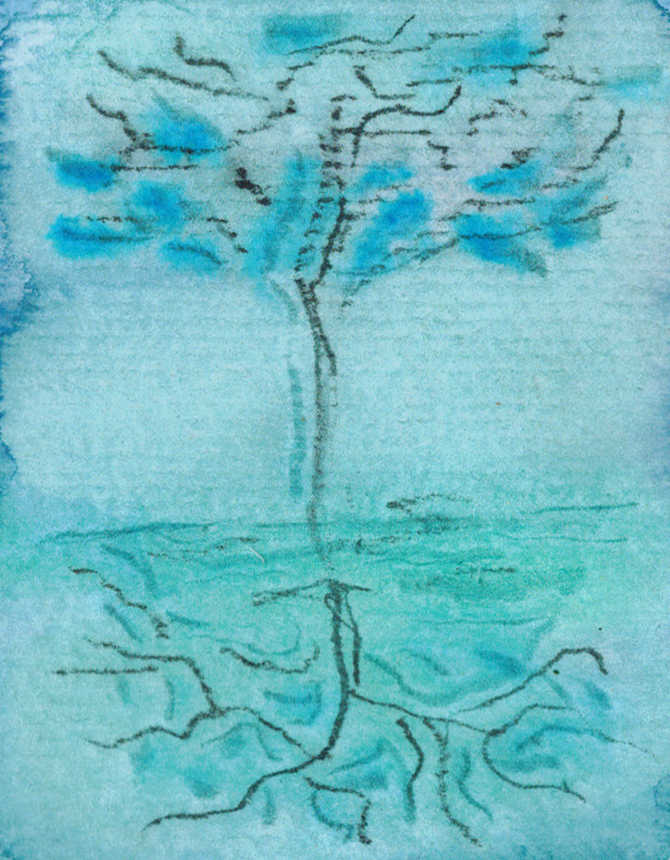
\includegraphics[scale=1.8]{./ethique/arbre}
\end{center}

\vfill

